{\justifying
	\chapterauthor{Brayan Riveros}%Puede ser nombre simplificado
	\chapter{Preparación de la plantilla}
	\section{Copia de trabajo de GitHub (FORK)}
	Primero hacemos un FORK con nuestras cuentas personales de GitHub del siguiente repositorio
	\begin{center}
		\href{https://github.com/LosAcademycos/revistaMathUD/} {https://github.com/LosAcademycos/revistaMathUD/}
	\end{center}
	Luego hacemos una copia de trabajo en nuestros equipos, para ello abrimos una terminal Bash en la carpeta que deseemos y escribimos el siguiente comando 
	\begin{tcblisting}{terminal, terminal={$<$UsuarioGitHuB$>$ aquí va su usuario de GitHub}}
		git clone https://github.com/<UsuarioGitHuB>/revistaMathUD/ 
	\end{tcblisting}
	Entramos a la capeta de la plantilla con el siguiente comando
	\begin{tcblisting}{terminal, terminal={En esta carpeta ejecutaremos todos los comandos git}}
	cd revistaMathUD
	\end{tcblisting}
	Lo primero que debemos haces es ubicarnos en la rama template, con el siguiente comando 
	\begin{tcblisting}{terminal, terminal={El comando git checkout es de los más básicos de git}}
		git checkout template
	\end{tcblisting}
	Aquí crearemos una rama con el nombre del artículo usando lowerCamelCase ver la sección \ref{sec:estandares} del capítulo \ref{cap:guiaDeUsuario}
	\begin{tcblisting}{terminal, terminal={Este comando es una abreviación de branch y checkout}}
		git checkout -b <nombreDeArticulo>
	\end{tcblisting}
	\begin{mybox}[A modo de ejemplo...]
		De aquí en adelante a modo de ejemplo supondremos que nuestro articulo se llama Ecuación de difusión, así que la rama se llama ecuacionDeDifusion
	\end{mybox}
	Como la rama recién creada depende de template, allí encontraremos un archivo baseArticulo.zip, descomprimimos el archivo y lo combinamos con la carpeta revistaMathUD. Y hacemos los siguientes pasos
	\begin{enumerate}
		\item Cambie el nombre de la carpeta NAMEARTICLE ubicada en articles/ por el nombre de su articulo \comillas{ecuacionDeDifusion} (este nombre, es solo a modo de ejemplo).
		\item Cambie el nombre del archivo BOOKS.bib ubicado en la carpeta references/ por el nombre del articulo \comillas{ecuacionDeDifusion} (no olvide que el formato debe quedar .bib) este será el archivo de su bibliografía, también cambie el nombre del archivo ARTICLE.tex por el de su artículo \comillas{ecuacionDeDifusion}.
		\item Abra el archivo load.tex ubicado en la carpeta antigua NAMEARTICLE, y el archivo antiguo ARTICLE.tex.
		y busque y reemplace el texto $<$carpetaArticulo$>$ por el nombre de su artículo \comillas{ecuacionDeDifusion}.
		\item Abra el archivo article.tex ubicado en la carpeta antigua NAMEARTICLE y modifique los datos $<$autor$>$, $<$nombreDelArticulo$>$, $<$autorNombreCompleto$>$, $<$correoElectronico$>$, $<$universidad$>$.
		\begin{mybox}[Nota]
			Si el artículo es de varios autores, consulte el capitulo \ref{cap:guiaDeUsuario}.
		\end{mybox}
		\item Compile el archivo antiguo main.tex en este caso llamado \comillas{ecuacionDeDifusion.tex}, siguiendo las instrucciones de la sección \ref{sec:compilacion}, es normal que la bibliografía compile con un error debido al paquete \verb|bibunits|.
		\begin{mybox}[Nota]
			No puede existir ningún otro tipo de error diferente a la compilación de la bibliografía.
		\end{mybox}
	\end{enumerate}
	\section{Errores comunes}
	La mayoría de errores se debe a la distribución del {\LaTeX} (MiKTeX o TeXLive) que no esta actualizada, si esta trabajando en Linux, mediante uso de la terminal puede actualizar el TeXLive. Para MiKTeX lo puede actualizar desde la aplicación MiKTeX Console.
	\begin{mybox}[Recomendación]
		Antes de compilar la plantilla, asegúrese de tener la distribución del {\LaTeX} actualizada.
	\end{mybox}
	\section{Compilación}\label{sec:compilacion}
	Una vez actualizado la distribución del LaTeX (MiKTeX – TeXLive) debemos descargar e instalar TeXstudio (https://www.texstudio.org/) y procedemos a configurar el TeXstudio (se configura de manera similar el TeXMaker), para ello vamos a 
	\begin{center}
		opciones -> configurar TeXstudio -> pestaña órdenes.
	\end{center}
	En PdfLaTeX debe tener esta línea de comando
	\begin{center}
		pdflatex.exe --shell-escape -synctex=1 -interaction=nonstopmode \%.tex
	\end{center}
	normalmente solo se debe agregar --shell-escape, también debemos configurar la orden del BibTeX, para en la misma pestaña órdenes en BibTeX debe ir esta línea de comando
	\begin{center}
		bibtex ?me*/*.aux
	\end{center}
	y además debemos verifiquar que en la pestaña Compilar la herramienta bibliográfica por defecto sea BibTeX, con esto la plantilla debe compilar perfectamente con los botones \comillas{compilar} y \comillas{compilar \& ver} recuerde que con F8 compila la bibliografía. En resumen, la compilación debe ser 
	\begin{center}
		PdfLaTeX -> BibTeX -> PdfLaTeX
	\end{center}
	\begin{mybox}[Nota]
		Para mayor velocidad de compilación debemos desmarcar las opciones de repetir las órdenes de compilación contenidas (debemos marcar la opción Mostrar opciones avanzadas) en
		\begin{center}
			Órdenes -> PdfLaTeX\\
		    Compilar -> Compilador por defecto.
		\end{center}
		Aunque recuerda que algunas características deben compilarse dos veces.
	\end{mybox}
	
}\cleanalldata
{\justifying
	\chapterauthor{Brayan Riveros}%Puede ser nombre simplificado
	\chapter{Guía de usuario}\label{cap:guiaDeUsuario}
	\section{Artículo personalizado}
	Antes de iniciar la redacción de cualquier articulo entendamos la estructura básica del artículo
	\begin{tcblisting}{boxlatex}
	{\justifying
		\chapterauthor{<Autor>}
		\chapter{<nombre del articulo>}\label{art:<nombre del articulo upperCamelCase>}
	}\cleanalldata
	\end{tcblisting}
	Los siguientes datos son los que se mostrarán en el encabezado del artículo
	\begin{center}
		<autor>  = Nombre del autor, como guste el autor.\\  
		<nombre del articulo> = Es el nombre del artículo completo.\\
	\end{center}
	El comando \verb|\label| es la referencia del artículo y debe tener la estructura mostrada en el código anterior.\pap
	El primer contenido de cualquier artículo es la ficha técnica del autor y el abstract, para ello disponemos de comandos y entornos preestablecidos
	\begin{tcblisting}{boxlatex}
		\infoauthorarticle{}{}{}
		\begin{infoauthorarticlebox}
		\end{infoauthorarticlebox}
		\begin{abstract}
		\end{abstract}		
	\end{tcblisting}
	Veamos el funcionamiento de cada uno de ellos, si el artículo es realizado por un solo autor, el comando \verb|\infoauthorarticle| es el indicado, donde los argumentos son el nombre completo, correo y universidad, por ejemplo
	\begin{tcblisting}{boxlatex}
		\infoauthorarticle{Brayan Camilo Riveros Castellanos}{camilor2611@gmail.com}{Universidad Distrital Francisco José de Caldas}	
	\end{tcblisting}
	Cuyo resultado es
	\infoauthorarticle{Brayan Camilo Riveros Castellanos}{camilor2611@gmail.com}{Universidad Distrital Francisco José de Caldas}
	Si el artículo es de varios autores debemos utilizar el entorno \verb|infoauthorarticlebox|, por ejemplo un artículo con dos autores de la misma universidad
	\begin{tcblisting}{boxlatex}
	\begin{infoauthorarticlebox}
		\faPencil\hspace{5pt} Brayan Camilo Riveros Catellanos.\\
		\faAt\hspace{9pt}\href{mailto:camilor2611@gmail.com} {camilor2611@gmail.com}.\\
		\faPencil\hspace{5pt} Kevin Sebastián Pineda Jaramillo.\\
		\faAt\hspace{9pt}\href{mailto:kevin961312@gmail.com} {kevin961312@gmail.com}.\\
		\faUniversity\hspace{2pt} Universidad Distrital Francisco José de Caldas.
		\tcblower
		\tcbincludegraphics[transparent, marginsInteriorNull, graphics options={width=2cm}]{png/users.png}
	\end{infoauthorarticlebox}
	\end{tcblisting}
	Cuyo resultado es
	\begin{infoauthorarticlebox}
		\faPencil\hspace{5pt} Brayan Camilo Riveros Catellanos.\\
		\faAt\hspace{9pt}\href{mailto:camilor2611@gmail.com} {camilor2611@gmail.com}.\\
		\faPencil\hspace{5pt} Kevin Sebastián Pineda Jaramillo.\\
		\faAt\hspace{9pt}\href{mailto:kevin961312@gmail.com} {kevin961312@gmail.com}.\\
		\faUniversity\hspace{2pt} Universidad Distrital Francisco José de Caldas.
		\tcblower
		\tcbincludegraphics[transparent, marginsInteriorNull, graphics options={width=2cm}]{png/users.png}
	\end{infoauthorarticlebox}
	Por lo que la estructura inicial del artículo es
	\begin{tcblisting}{boxlatex}
	{\justifying
		\chapterauthor{<autor>}%Puede ser nombre simplificado
		\chapter{<nombreDelArticulo>}
		\infoauthorarticle{<autorNombreCompleto>}{<correoElectronico>}{<universidad>}
	}\cleanalldata	
	\end{tcblisting}
	Claramente el entorno \verb|abstract| nos permitirá escribir el resumen de nuestro articulo dando como resultado
	\begin{abstract}
		\lipsum[1]
	\end{abstract}
	\begin{mybox}[Nota]
		El comando \verb|\cleanalldata| es necesario para la fase de producción de la revista, no se puede eliminar, al igual que el comando \verb|{\justifying}| cuyo funcionamiento es justificar el texto.
	\end{mybox}
	\subsubsection{Opcionales}
	Si queremos agregar un epigrafo agregamos una linea de código similar a la siguiente después de \verb|\chapter|.
	\begin{tcblisting}{boxlatex}
		\epigraph{\comillas{Es perfectamente obvio que el mundo entero se va al infierno. La única oportunidad posible es que procuremos que no sea así}}{--- \textup{Robert Oppenheimer}}
	\end{tcblisting}
	También podemos agregar una imagen representativa esto lo hacemos definiendo la ruta de la imagen antes de \verb|\chapter|.
	\begin{tcblisting}{boxlatex}
		\chapterimage {<pathImagesCommand>/chapter/<nombreImagen>} {3cm}
	\end{tcblisting}
	Ejemplo 
	\begin{tcblisting}{boxlatex}
	{\justifying
		\chapterimage{chapter/Bomba.jpg}{3cm}
		\chapterauthor{Brayan Riveros \& Kevin Pineda}
		\chapter{Ecuaciones de difusión, reacción y deriva}\label{art:EcuacionesDeDifusiónReacción}
		\epigraph{\comillas{Frase}}{--- \textup{autor}}
		\begin{abstract}
			contenido
		\end{abstract}
	}\cleanalldata
	\end{tcblisting}
	\newpage
	\section{Bibliografía}
	La bibliografía se recomienda trabajarla con JabRef, lo importante de esta parte del artículo son las bibtexkey, ya que el compilador puede encontrar dos iguales y pasarla como advertencia. Para mantener un estándar la bibtexkey debe tener la siguiente estructura
	\begin{tcblisting}{boxlatex}
	 	bib:<nombre de libro o autor en upperCamelCase> 
	 	%----- o de manera alterna......
	 	book:<nombre de libro en upperCamelCase> 
	\end{tcblisting}
	Por ejemplo la bibtexkey es \verb|bib:ecuacionesDiferenciales|
	lo podemos citar con el comando típico
	\begin{tcblisting}{boxlatex}
		\cite{bib:ecuacionesDiferenciales}
	\end{tcblisting}
	Para mostrar la bibliografía agregamos el comando \verb|\putbib| entre \verb|\justifying|, por ejemplo
	\begin{tcblisting}{boxlatex}
		{\justifying
		Contenido de artículo... 
		\putbib
		}\cleanalldata
	\end{tcblisting}
	\newpage
	\section{Entornos}
	Los siguientes entornos tienen dos argumentos obligatorios, si no se desea utilizar los argumentos se deben dejar en blanco, esto es \{\}\{\}. El primer argumento es el nombre del entorno y el segundo es la llave (key) de la referencia, vemos los entornos más usuales. 
	\begin{tcblisting}{boxlatex}
		\begin{mylem}{Lema de Zorn}{lemaZorn}
			Contenido lema
		\end{mylem}
		Para referenciar el lema se utiliza \ref{lem:lemaZorn}
	\end{tcblisting}
	Ejemplo
	\begin{mylem}{Lema de Zorn}{lemaZorn}
		Contenido lema
	\end{mylem}
	Según el lema \ref{lem:lemaZorn} obtenemos ...
	\begin{tcblisting}{boxlatex}
		\begin{mytheo}{Teorema de pitágoras}{pitagoras}
			Contenido teorema
		\end{mytheo}
		Para referenciar el teorema se utiliza \ref{theo:pitagoras}
	\end{tcblisting}
	Ejemplo
	\begin{mytheo}{Teorema de pitágoras}{pitagoras}
		Contenido teorema
	\end{mytheo}
	Según el teorema \ref{theo:pitagoras} concluimos...\pap
	\begin{tcblisting}{boxlatex}
		\begin{mydef}{Dominio entero}{domEntero}
			Contenido definición
		\end{mydef}
		Para referenciar la definición se utiliza \ref{def:domEntero}
	\end{tcblisting}
	Ejemplo
	\begin{mydef}{Dominio entero}{domEntero}
		Contenido definición
	\end{mydef}
	Según la definición \ref{def:domEntero} es claro que ...\pap
	De manera similar funcionan lo siguientes entornos
	\begin{tcblisting}{boxlatex}
		%-------Corolario-----------
		\begin{mycor}{Nombre corolario}{nom}
			Contenido corolario
		\end{mycor}
		Para referenciar el corolario se utiliza \ref{cor:nom}
		%------propiedades----------
		\begin{myprop}{números reales}{numReales}
			Contenido propiedades
		\end{myprop}
		Para referenciar las propiedades se utiliza \ref{prop:numReales}
		%---------definición---------
		\begin{mydef}{Dominio entero}{domEntero}
			Contenido definición
		\end{mydef}
		Para referenciar la definición se utiliza \ref{lem:domEntero}
		%------proposición-----------
		\begin{myproposi}{}{nomProposicion}
			Contenido proposición
		\end{myproposi}
		Para referenciar la proposición se utiliza \ref{proposi:nomProposicion}
	\end{tcblisting}
	Otros entornos predefinidos son
	\begin{tcblisting}{boxlatex}
		\begin{mynote}
			Contenido nota
		\end{mynote}
		%---------caja------------
		\begin{mybox}[<título>]
			Contenido caja
		\end{mybox}
		%-----------tabla----------
		\begin{mytable}[tabularx={X|X|X}, width=10cm]{<título>}
			cell A & Cell B & Cell B\\\hline
			cell C & Cell D & Cell B
		\end{mytable}
	\end{tcblisting}
	\newpage
	\section{Estándares}\label{sec:estandares}
	Antes de mencionar de los estándares del código de esta revista, tenga en cuenta que no son obligatorios, pero seguirlo puede evitar trabajo tanto para los productores de la revista como los autores, sin mas preambulo veamos que es la notación Camel Case\pap 
	Camel case es una notación que nos permite nombrar las variables, funciones o clases en un lenguaje de programación, esta a su vez se divide en dos casos UpperCamelCase y lowerCamelCase.\pap
	\textbf{UpperCamelCase}.
	La escritura utilizando UpperCamelCase es iniciar en mayúscula cada palabra que compone el nombre de la variable, sin olvidar que esta no puede tener espacios ni caracteres especiales.\pap 
	\textbf{lowerCamelCase}.
	La escritura utilizando lowerCamelCase es iniciar en minúscula cada palabra que compone el nombre de la variable, sin olvidar que esta no puede tener espacios ni caracteres especiales.
	\subsubsection{Comandos}
	Recuerde que la estructura de un comando es:
	\begin{center}
		\begin{tcblisting}{boxlatex}
			\newcommand{\<nombre>}[<arguments number>]{<function>}
		\end{tcblisting}
	\end{center}
	Para nombrar correctamente los comandos se usará la notación lowerCamelCase
	\subsubsection{Referencias}
	Todas las referencias de la mayor parte de los entornos tienen un prefijo, esto conlleva a una buena organización y previene el error de referencias iguales para entornos diferentes.
	\begin{mybox}[Convención]
		Algunas referencias no dependen da la plantilla como lo es el caso de los artículos y ecuaciones, por ello se recomienda seguir el siguiente  estándar: 
		\begin{itemize}
			\item Artículo. \verb|\label{art:<nombre>}|.
			\item Sección. \verb|\label{sec:<nombre>}|
			\item Ecuación. \verb|\label{eqn:<nombre>}|.
			\item Item. \verb|\label{itm:<nombre>}|.
			\item Imagen. \verb|\label{fig:<nombre>}|.
			\item Bibliografía. \verb|\label{bib:<nombre>}| o \verb|\label{book:<nombre>}|.
			\item Tabla. \verb|\label{tab:<nombre>}|.
		\end{itemize}
		\begin{mynote}
			Para el \verb|<nombre>| utilizaremos la estandarización lowerCamelCase. 
		\end{mynote}
	\end{mybox}
	\subsubsection{Estándar de nombres de archivos}
	Para los nombres de todos los archivos del autor (incluyendo imágenes y código \LaTeX) no se utilizará espacios ni caracteres especiales, entonces seguiremos el siguiente estándar: 
	\begin{center}
		\textbf{algebraLineal.tex} o \textbf{cuboRubik.png.}
	\end{center}
	Obsérvese que se usa la notación lowerCamelCase.
	\begin{mynote}
		Los nombres de los archivos utiliza el idioma en el que esta redactado el artículo.
	\end{mynote}
	\section{Revista (Divulgación)}
		Debido a las librerías utilizadas en la programación de la plantilla podemos crear unos covers similares a revistas divulgativas. Al ser un diseño dependiente del creador la mayor parte de variantes deben ser modificadas manualmente, se recomienda activar el comando \verb|\BgThispage| de el plugin \textbf{marginsPrint}.
	\newpage
	\section{Código}
	Este código utilizar el entorno \textbf{coverpage}.
	\begin{tcblisting}{boxlatex}
		\begin{coverpage}
			\AddToShipoutPicture*{\put(-400,-100){
					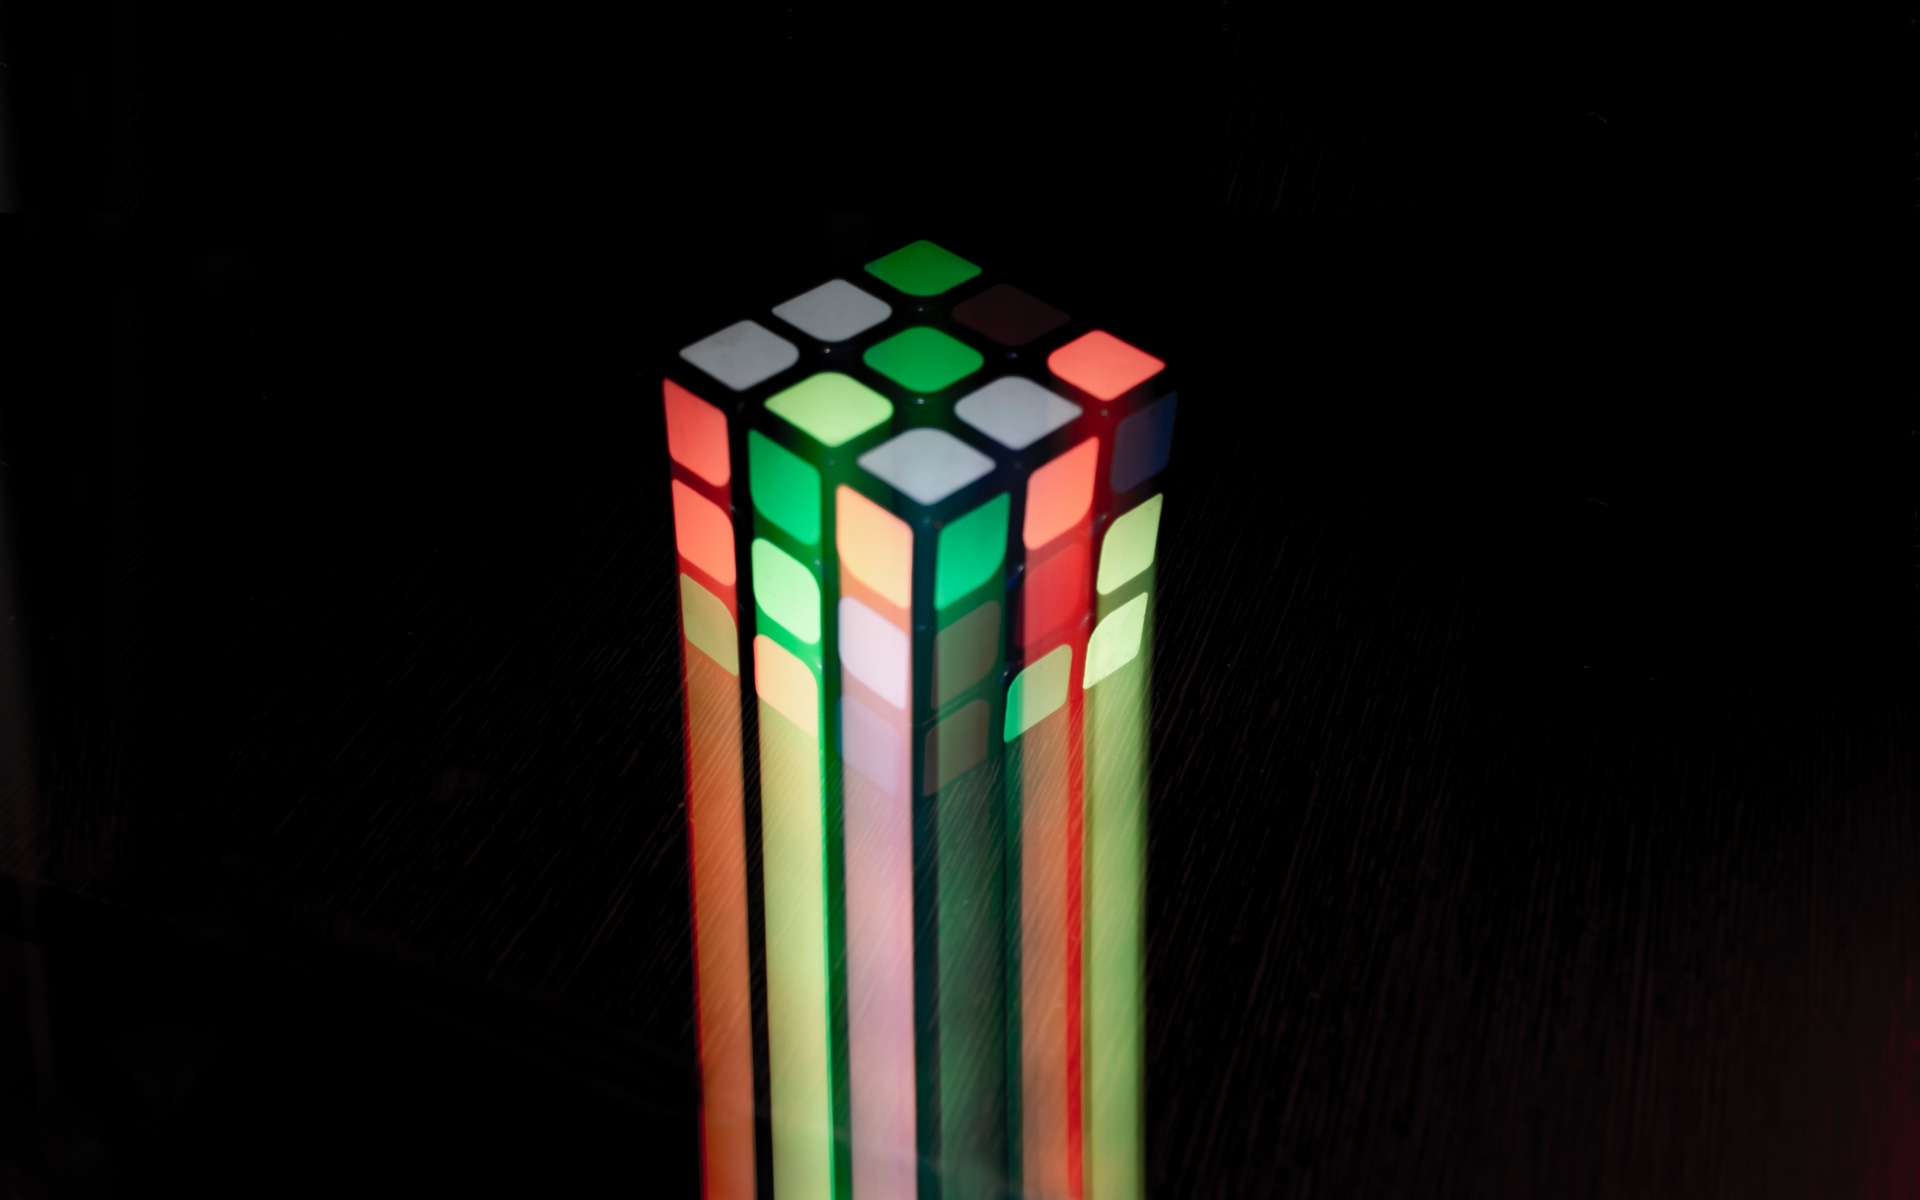
\includegraphics[scale=1]{\usersGuideImages/jpg/rubiksCube.jpg}
				}
			}
			\put(180,0){
				\begin{tcolorbox}[boxPrimaryMagazineStyle1, height=\textheight, width = 7.5cm]
					Texto						
				\end{tcolorbox}  
			}
		\end{coverpage}
	\end{tcblisting}
	\newpage
	\begin{coverpage}
		\AddToShipoutPicture*{\put(-400,-100){
				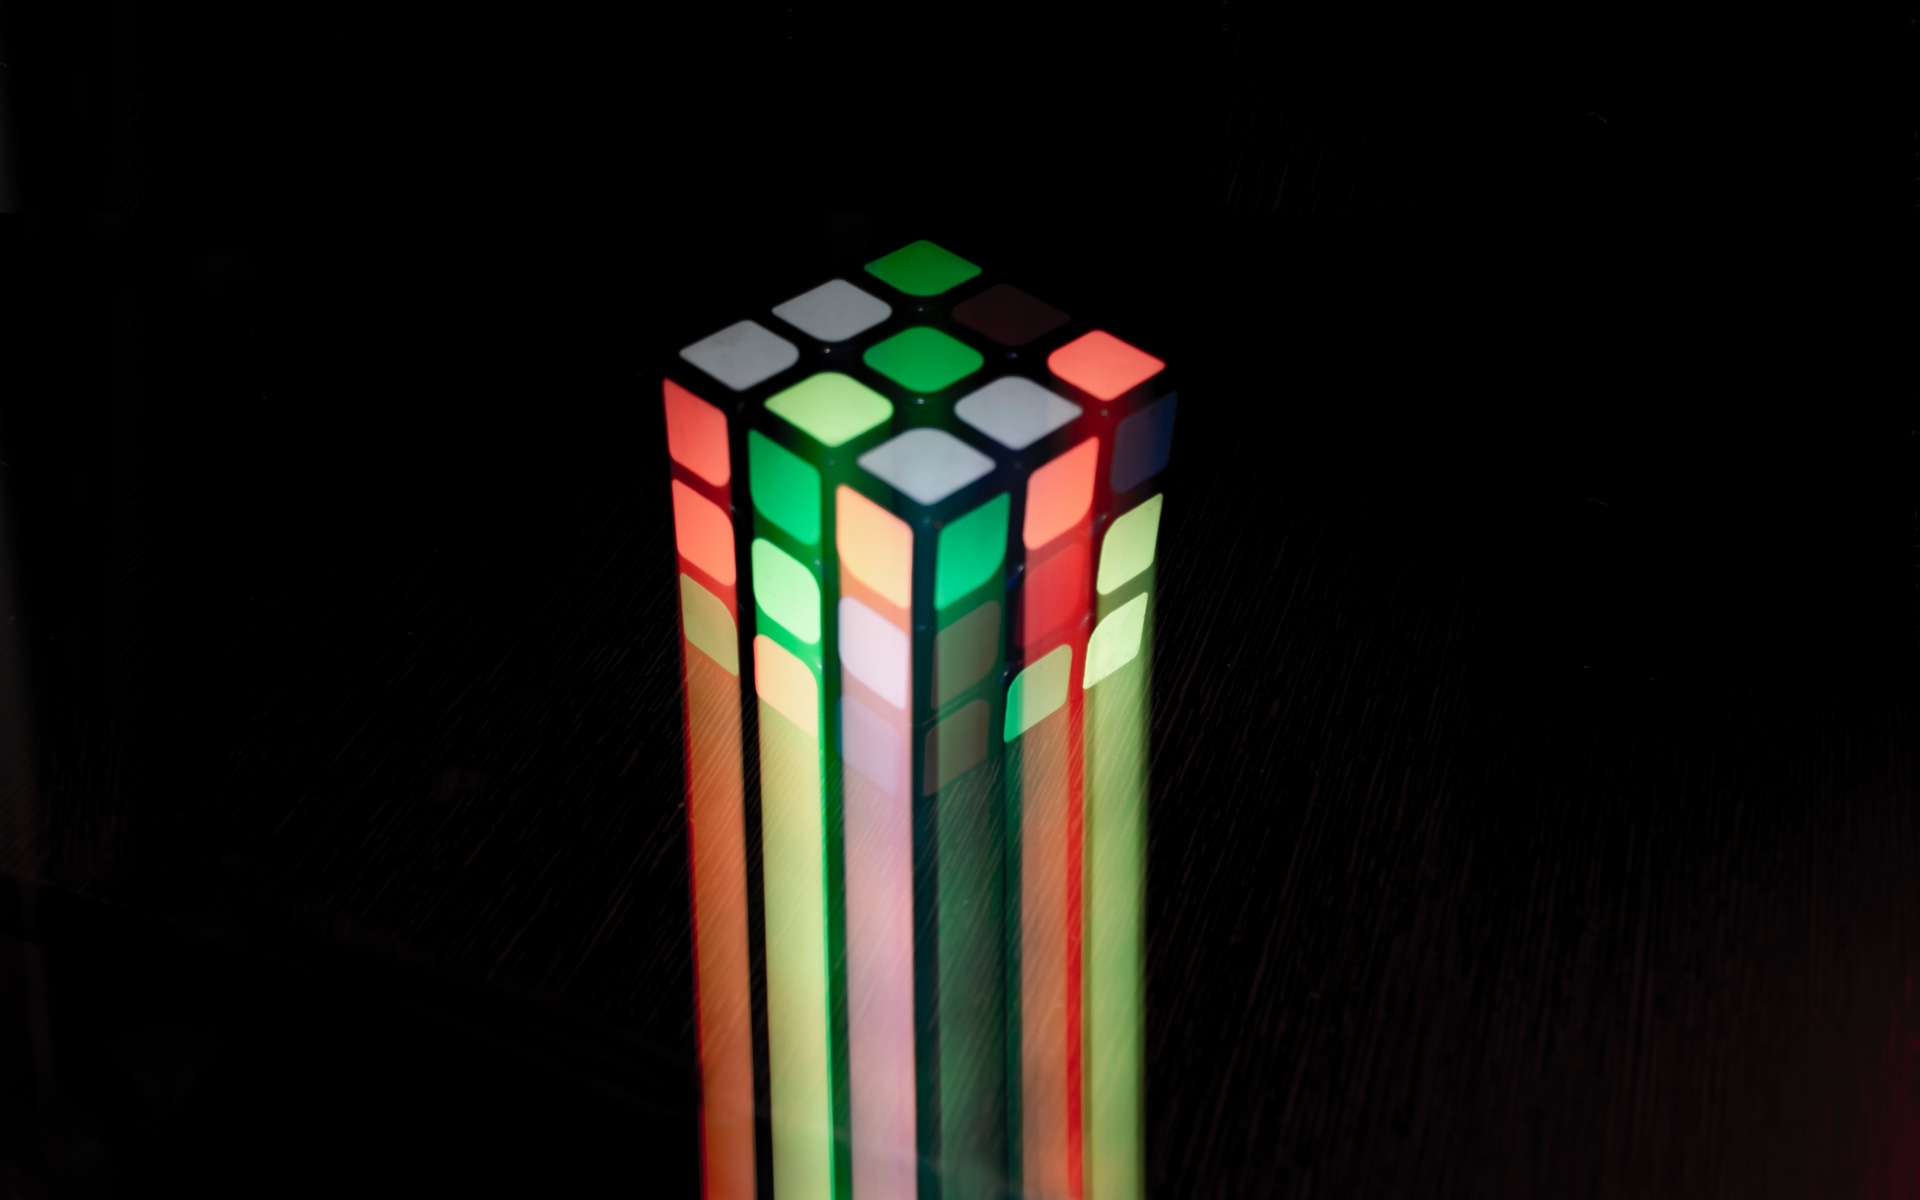
\includegraphics[scale=1]{\usersGuideImages/jpg/rubiksCube.jpg}
			}
		}
		\put(180,0){
			\begin{tcolorbox}[boxPrimaryMagazineStyle1, height=\textheight, width = 7.5cm]
				{\Huge Cubo de Rubik}\\ \\
				Un cubo de Rubik clásico posee seis colores uniformes (tradicionalmente blanco, rojo, azul, naranja, verde y amarillo). Un mecanismo de ejes permite a cada cara girar independientemente, mezclando así los colores. Para resolver el rompecabezas, cada cara debe volver a quedar en un solo color.
				\\ \\
				El cubo celebró su 25. aniversario en 2005, por lo que salió a la venta una edición especial del mismo en la que la cara blanca fue remplazada por una reflectante en la que se leía Rubik's Cube 1980-2005. En su 30. aniversario, en 2010, se comercializó otra edición especial fabricada en madera.
				\\ \\
				Existen variaciones con diversos números de cuadrados por cara. Las principales versiones que hay son las siguientes: el 3×3×3, el cubo de Rubik estándar (el 4×4×4 (La venganza de Rubik), el 5×5×5 (El cubo del profesor); y desde septiembre de 2008 el 6×6×6 (V-Cube 6) y el 7×7×7 (V-Cube 7) de Verdes Panagiotis La empresa Shengshou lanzó al mercado a principios de 2012 cubos de 8x8x8, 9x9x9 y 10x10x10.
			\end{tcolorbox}  
		}
	\end{coverpage}
	\newpage
	\BgThispage
	\begin{coverpage}
		\AddToShipoutPicture*{\put(-300,-200){
				
\includegraphics[scale=1]{\usersGuideImages/jpg/rubiksCube2.jpg}
			}
		} 
		\put(180,0){
			\begin{tcolorbox}[boxPrimaryMagazineStyle1, height=\textheight, width = 7.5cm
				]
				{\Huge Cubo de Rubik}\\ \\
				Un cubo de Rubik clásico posee seis colores uniformes (tradicionalmente blanco, rojo, azul, naranja, verde y amarillo). Un mecanismo de ejes permite a cada cara girar independientemente, mezclando así los colores. Para resolver el rompecabezas, cada cara debe volver a quedar en un solo color.
				\\ \\
				El cubo celebró su 25. aniversario en 2005, por lo que salió a la venta una edición especial del mismo en la que la cara blanca fue remplazada por una reflectante en la que se leía Rubik's Cube 1980-2005. En su 30. aniversario, en 2010, se comercializó otra edición especial fabricada en madera.
				\\ \\
				Existen variaciones con diversos números de cuadrados por cara. Las principales versiones que hay son las siguientes: el 3×3×3, el cubo de Rubik estándar (el 4×4×4 (La venganza de Rubik), el 5×5×5 (El cubo del profesor); y desde septiembre de 2008 el 6×6×6 (V-Cube 6) y el 7×7×7 (V-Cube 7) de Verdes Panagiotis La empresa Shengshou lanzó al mercado a principios de 2012 cubos de 8x8x8, 9x9x9 y 10x10x10.
			\end{tcolorbox}  
		}
	\end{coverpage}
	
%	\putbib % muestra la bibliografia
}\cleanalldata	